\chapter*{Ninguém está a salvo, muito menos o poeta}
\addcontentsline{toc}{chapter}{Ninguém está a salvo, muito menos o poeta, \emph{por Alcir Pécora}}

\begin{flushright}
\emph{Alcir Pécora}
\end{flushright}

Não sei bem dizer o que ouço. Difícil até saber o que ouço ao ouvir
\emph{Álbum -- Deus devolve o revólver}, de Régis Bonvicino.

\emph{Streaming} de poesia com tratamento sonoro talvez fosse o mais
descritivo a dizer. O poeta Régis Bonvicino reúne aqui 16 novos poemas
--, lidos por ele, pela soprano Caroline De Comi e pelo poeta
norte-americano Charles Bernstein --, trabalhados sonoramente por
Rodrigo Dário, que também cuidou de todo o \emph{design} da empreitada,
incluindo a bela e anacrônica fita K"-7, um dos suportes físicos
previstos para \emph{Deus devolve o revólver}, além de um libreto ao
feitio de ópera.

A qualidade da poesia, por si mesma, é extraordinária -- eis o que
precisa ser dito antes de mais nada. Para sentir a potência literária
dela bastaria que fosse lançada como livro, o que deverá ocorrer no
próximo ano, incluindo um número bem maior de poemas. Mas convém
ressaltar também a felicidade desse encontro entre Régis e Bernstein,
seu parceiro de outras lides, e seus dois jovens parceiros paulistanos,
advindos de outras áreas artísticas: Rodrigo, artista plástico,
\emph{design} gráfico e de som; Caroline, soprano colatura, sem os quais
isso que ouço não seria jamais o mesmo que ouço. Embora jovens, está
claro que ambos demonstram talento e abertura para a criação radical,
associados a um grande apuro técnico. Algo novo se gestou entre eles: um
álbum de poesia eletrônica \emph{heavy}.

Os poemas, vale avisar, são muito duros.

Poemas de mastigar pedras -- não as dos agrestes, como as de
Cabral, ou as de ferro, como as de Drummond, mas é óbvio que o
construtivismo do primeiro, como o desengano lírico do segundo são um
legado decisivo para a poesia de Régis. Poemas de mastigar ruínas dos
centros das grandes cidades brasileiras, de que São Paulo é o exemplo
por antonomásia, tendo por centro os seus acampamentos ubíquos de
lumpens, cuja figura mais desamparada e fora de controle, mais
impossível de assimilar à vida civil, é o \emph{noia}. Cerca"-o uma
muralha da classe média empobrecida, igualmente agressiva, e ilhas de
riqueza fora da lei, cujo delírio é pensar que estão no golfo de Miami,
quando não nas praias vermelhas de Marte.

A contundência física da metrópole falida (e não o seu diagnóstico
abstrato) é o assunto minuciosamente esquadrinhado por Régis: maus
cheiros, maus"-tratos, maus bofes, os habitantes habitualmente fora de
si, movimentos bruscos, presenças inconvenientes que ocupam todos os
buracos da metrópole sul"-americana precocemente arruinada. Tudo aqui
demonstra ostensivamente o cerne falido do Brasil como projeto
civilizatório europeu.

Nesses poemas de horror -- não sei de maneira mais exata de
caracterizá-los --, nos quais ninguém está a salvo, muito menos o poeta,
exposto a tudo que vê e anota, a falência se diz de muitas maneiras:
pela indiferença ao sofrimento alheio, e, ainda mais, pelo gosto sensual
do sofrimento alheio; pela expansão tóxica da corrupção financeira; pela
ação abjeta da indústria farmacêutica, que faz da fragilidade psíquica o
coração de seu negócio; pelo amor ao Deus fundamentalista e midiático,
aliado de toda violência contra os que não partilham da mesma Glória da
ignorância; pelo cuidado minucioso com a lavagem de palavras cruas, que
tinham ao menos a vantagem de evidenciar as contradições de seus usos,
por outras, higienizadas segundo o processo do \emph{doublethink} que
faz do passado uma mera contingência dos negócios do presente etc. etc.
Não há descanso, não há faixas de repouso na poesia barra-pesada de
Régis Bonvicino.

Mas isso são apenas sentidos gerais, e a poesia é, antes de tudo,
experiência do particular.

Os poemas de Régis Bonvicino, na forma mais direta de descrevê"-los
tecnicamente, apresentam ondas sucessivas de écfrases paratáticas,
descrições e colagens de corte seco de cenas de rua da megalópole, cujo
protagonismo forçado, \emph{gauche}, cabe desde logo aos mendigos. Das
écfrases, Régis explora notadamente duas direções: de um lado, a das
contradições em relação aos enunciados da política neoliberal, em que a
riqueza é entendida como multiplicação da pobreza, e o investimento como
operação inalterada por mãos humanas.

De outro lado, o que é mais surpreendente e o que, em geral, reserva
para o fecho dos poemas, Régis desenvolve a ideia de que toda a miséria
visível está reconstruída em nossas mentes como roteiro de um
\emph{reality show} monstruoso, de cuja existência os poemas apenas
chegam a ser pistas. As histórias de vida, nesse caso, não surgem como
experiência real de seres destruídos pela história, mas sim como efeito
de uma inércia narrativa que remete à própria composição do poema. Isto
é, a poesia que se lê é a poesia que lida com a sua fatalidade própria,
de iluminar vidas perdidas, destinos miseráveis, situações abjetas a que
está obrigada a anotar, sem escapatória. Em suma, como condenação que
está obrigada a encenar e que finalmente se abate sobre si mesma: fazer
poesia como acender a sua pedra e consumi"-la, como poesia da desgraça
própria e intransferível.

Em ambas as direções, a da contradição histórica e a da condição
terrível em que nasce a poesia de Régis Bonvicino, o tratamento
eletrônico de Rodrigo Dário, cuja origem parece estar no
\emph{industrial rock} dos anos 1990, acentua uma espécie de urgência
paradoxal em meio ao vazio e à desolação já instalados. Alertas e
sirenes disparam sobre um maquinismo monocórdio, grave/agudo, recitado,
atrofiado. Ecos reverberam ameaçadores sobre uma paisagem distópica. A
poesia de Régis, nesse estranho álbum, ganha qualquer toque lynchiano,
que acentua muito apropriadamente a sua natureza quebrada, sombria e
catastrófica.

\pagebreak
\thispagestyle{empty}
%\part{LADO A}

\begin{absolutelynopagebreak}
%\thispagestyle{empty}

\begin{vplace}
\begin{figure}[H]
\begin{adjustwidth}{-3cm}{}
  %\centering
  \vspace*{14.7cm}
  %\hspace{-0.5cm}
  \includegraphics[width=140mm]{./LADO_A.pdf}  
  %\hfill
\end{adjustwidth}

\end{figure}
\end{vplace}

\end{absolutelynopagebreak}

\addcontentsline{toc}{part}{Lado A}
\chapter*{LADO A}
\addcontentsline{toc}{chapter}{\textbf{A nova utopia (1)}\\ Lido por Régis Bonvicino}
\textbf{A nova utopia (1)}\\
Lido por Régis Bonvicino

\bigskip

A nova utopia é uma borboleta negra, desatenta, com olhos exuberantes. A
nova utopia é a favor da proteção implacável dos animais. A nova utopia
é inclusiva, participativa. A nova utopia é o coro afinado dos
descontentes. É um ex-guerrilheiro, de porte avantajado, homem forte do
governo. A nova utopia tem informações privilegiadas, disponíveis. É um
ex-leproso. A nova utopia rechaça a figura de Nossa Senhora se
masturbando. A nova utopia defende os direitos das trabalhadoras do
sexo. A nova utopia comunga, com moderação, ideais materialistas. A nova
utopia morre de pé. É, ao mesmo tempo, um \emph{duty free} e um
\emph{detox} financeiro. A nova utopia é nosso dever como cidadãos. A
nova utopia exalta a sustentabilidade das empresas. A nova utopia sabe
que se pode ser árabe e muçulmano, árabe e não muçulmano, muçulmano sem
ser árabe. Negro sem ser branco, branco sem ser negro. A nova utopia é a
liberdade de expressão do \emph{Le Monde}, reassegurada desde sempre. A
nova utopia é um ajuste de contas contra o obscurantismo dos outros. A
nova utopia rejeita factoides politicamente úteis. A nova utopia é um
pouco xiita, apenas quando estritamente inevitável. É um turista
americano visitando o Museu Abu Ghraib. A nova utopia tem logo e
\emph{slogan}. Condena chacinas na periferia. A nova utopia emite notas
de repúdio, lança abaixo-assinados; defende o grafite; a nova utopia
prega a bicicleta. A nova utopia é o respeito incondicional ao nanismo.
Condena corruptos. É um ex-ladrão. Tem seu próprio dicionário. Pensa
antes de agir. Repele palavras e pede ação. A nova utopia é um ex-coxo.
É a asa aberta do voo. É um \emph{showroom} de exuberâncias naturais. É
um céu com nuvens negras, sob controle. É uma estante de livros num
banheiro. É a viúva de Jorge Luis Borges detalhando seu processo de
criação. A nova utopia é um ex-macumbeiro, um ex-bêbado, é um ex-exu
sujo. É um branco de alma preta. A nova utopia é ainda o indígena de
tocheiro, fazendo política, diariamente, nas redes sociais. A nova
utopia é uma ex-esteticista de unhas postiças. É um espião trans pegando
sol num roteador. É um ex-selvagem. É uma ex-vadia. É um ex-puto. É uma
entendida. É um ex-pária. É uma míriade de franquias de poetas
premiados. É um poema à altura de seu tempo.

\pagebreak
\begin{absolutelynopagebreak}
\textbf{Vinheta 1:}
\addcontentsline{toc}{chapter}{\textbf{Vinheta (1)}\\ Lido por Régis Bonvicino}

``Boa noite. Deus devolve o revólver''

Lido por Régis Bonvicino


\thispagestyle{empty}

\begin{vplace}
\begin{figure}[H]
%\begin{adjustwidth}{-0.01cm}{}
  \centering
  \vspace*{4cm}
  %\hspace{-0.5cm}
  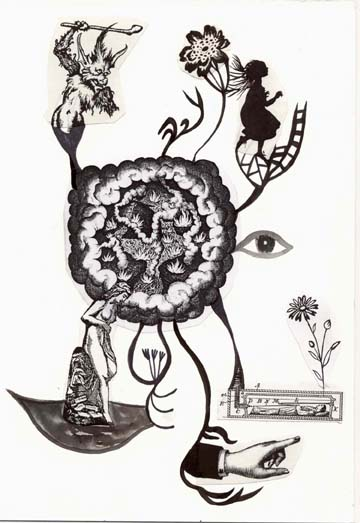
\includegraphics[width=100mm]{./imgs/caparc1.JPG}  
  %\hfill
%\end{adjustwidth}

\end{figure}
\end{vplace}

\end{absolutelynopagebreak}

\pagebreak

\textbf{Ficção}
\addcontentsline{toc}{chapter}{\textbf{Ficção}\\ Lido por Régis Bonvicino}

Lido por Régis Bonvicino

\begin{verse}
Pendurada de cabeça para baixo\\
via ao contrário a coluna em estilo coríntio\\
da antiga estação de trem\\
o poder político dos estoques\\[5pt]
as sacas de café, Bolsa de Nova York,\\
camionetes queimadas\\
um som adocicava o Largo\\
talvez fosse o de uma nova canção dos Beatles\\[5pt]
``Metralhado e morto outro facínora''\\
você com essa cara de filha de Maria\\
uma paulada na coluna\\
quebra as vértebras dessa puta\\[5pt]
boca fechada, o aparelho intacto\\
\emph{flashback} íntimo\\
o apontamento entre as páginas de um livro\\
o porta-malas do camburão\\[5pt]
as manchetes nas bancas\\
``O PIB vai a 10\%'',\\
``Prisioneiros viajam hoje'', alívio\\
baratas na vagina\\[5pt]
corte, tesoura, um talho no sutiã\\
tesoura roçando os seios\\
pode pisar neles\\
barata devidamente arquivada no cu\\[5pt]
o capuz, cabeça enfiada na água suja\\
os gritos sem porrada\\
ramos de café perfilam o capitel\\
portas maciças da altura do edifício Itália\\[5pt]
as teclas da pianola\\
em outro andar, mãos algemadas\\
nu na cadeira do dragão\\
o corpo do cara ficou odara
\end{verse}

\pagebreak

\textbf{Sermão}
\addcontentsline{toc}{chapter}{\textbf{Sermão}\\ Lido por Régis Bonvicino}

Lido por Régis Bonvicino

\begin{verse}
Uma \emph{joint-venture} de sem tetos, pele e osso, com medo da polícia, \qb{}aglomerada\\
no centro histórico de São Luís, mais de meia-noite, um dos mendigos, \qb{}bêbado, diz\\[15pt]
palavras ao vento\\
botaram Ford Landau no convento\\
padre não prega mais de costas --\\
contra -- como Vieira, mas de joelhos\\[5pt]
me ouçam logo de novo os peixes\\
tambor também não põe a mesa\\
galinha morta é veneno\\
o boi-bumbá só tem cordeiro\\[5pt]
para que serve tanto azulejo?\\
botaram mais um ladro no governo\\
urubu bica pedregulho\\
mato nasce em telhado\\[5pt]
o duque pega tudo\\
é bem mais de 10\%\\
lenda é passatempo\\
ganja é coisa de regueiro\\[5pt]
o mendigo há de subir\\
com o \emph{crack} na cabeça\\
moeda aqui cai somente no bueiro\\
escadaria é monumento\\[5pt]
miséria aqui é matinê\\
é bom guardar segredo\\
cavalo\\
não defeca mais dinheiro
\end{verse}

\pagebreak

\begin{absolutelynopagebreak}
\textbf{Vinheta 2:}
\addcontentsline{toc}{chapter}{\textbf{Vinheta (2)}\\ Lido por Régis Bonvicino}


\begin{verse}
``A mão que afaga é a mesma que apedreja\\
Apedreja essa mão vil que te afaga''\\[5pt]
Lido por Régis Bonvicino
\end{verse}

\thispagestyle{empty}

\begin{vplace}
\begin{figure}[H]
%\begin{adjustwidth}{-1.7cm}{}
  \centering
  \vspace*{2cm}
  %\hspace{-0.5cm}
  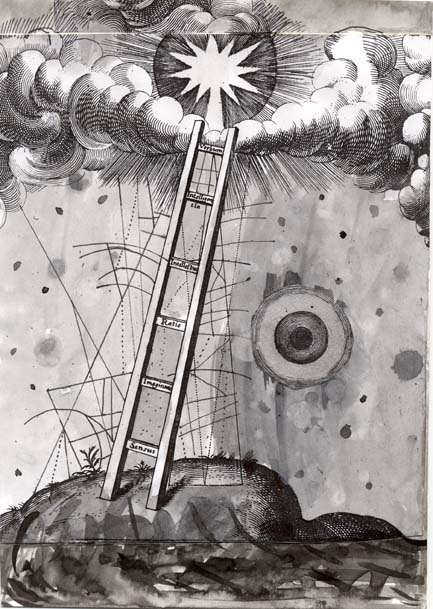
\includegraphics[width=100mm]{./imgs/caparc2.JPG}  
  %\hfill
%\end{adjustwidth}

\end{figure}
\end{vplace}

\end{absolutelynopagebreak}

\pagebreak

\begin{absolutelynopagebreak}
\textbf{Interlude}, Rodrigo Dário
\addcontentsline{toc}{chapter}{\textbf{Interlude (1)}\\ por Rodrigo Dário}

\thispagestyle{empty}

\begin{vplace}
\begin{figure}[H]
%\begin{adjustwidth}{-3.2cm}{}
  \centering
  \vspace*{3cm}
  %\hspace{-0.5cm}
  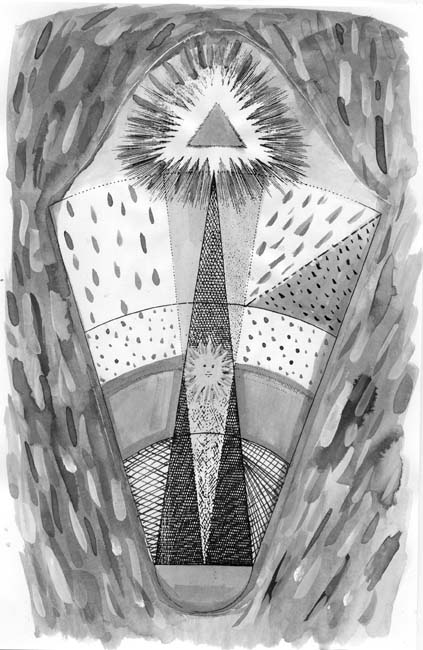
\includegraphics[width=100mm]{./imgs/caparc3.JPG}  
  %\hfill
%\end{adjustwidth}

\end{figure}
\end{vplace}

\end{absolutelynopagebreak}

\pagebreak

\textbf{Álibi}
\addcontentsline{toc}{chapter}{\textbf{Álibi}\\ Lido por Régis Bonvicino}

Lido por Régis Bonvicino

\begin{verse}
Oh, Pai, tende piedade\\
dos zilionários, dos vendedores legais de armas\\
dos lobistas, do dinheiro farto dos narcos\\
dos unhas de fome, dos gigolôs dos cassinos\\
dos traficantes de iguanas, rim e fígado\\[5pt]
Oh, Pai, tende piedade\\
dos banqueiros, dos juros sobre juros,\\
do laissez-faire chinês, do marketing do bem\\
dos plutocratas, dos fundos-abutres\\
garras, o condor-dos-andes não canta\\[5pt]
Oh, Pai, tende piedade\\
dos meões do dinheiro sujo dos contratos públicos\\
daqueles que depreciam os papéis de P.P. Pasolini\\
daqueles que lavam dinheiro com H. Matisse\\
misericórdia divina, delícia e êxtase dos santos\\[5pt]
Oh, Pai, tende piedade\\
dos xeques, dos grandes proprietários de terra\\
daqueles que não entregam a lebre\\
dos traficantes de marfim, caveiras com dentes e pedras\\
da criptomoeda, dos chefetes políticos despóticos\\[5pt]
Oh, Pai, tende piedade\\
dos traficantes de lixo eletrônico, dos agiotas\\
dos matadores de aluguel, dos guarda-costas\\
dos sócios ocultos, dos donos de \emph{offshores}\\
Oh, Pai, sobretudo tende piedade de nosso honrado \emph{boss}.
\end{verse}

\pagebreak

\textbf{Tarde}
\addcontentsline{toc}{chapter}{\textbf{Tarde}\\ Lido por Régis Bonvicino}

Lido por Régis Bonvicino

\begin{verse}
Junto ao muro arbustos, cactos\\
um deles, pontiagudo, alto,\\
avança na calçada\\
um grupo de nuvens cinza pesa\\
no ombro de uma mendiga negra que passa\\
poste, fios, janela, uma gambiarra\\
um carro pifado na guia\\
a um passo da avenida\\
parede de cubos de vidro\\
edifício, canteiro de espinhos,\\
dorme\\
estirado a uma certa distância da entrada\\
cabeça sobre a garrafa vazia de água\\
o sol de inverno bate direto em sua cara\\
roupas do corpo,\\
sem sapatos,\\
não tem mais nada, não tem \emph{spleen}\\
só tem porrada
\end{verse}

\pagebreak

\textbf{Perspectiva}
\addcontentsline{toc}{chapter}{\textbf{Perspectiva}\\ Lido por Régis Bonvicino}

Lido por Régis Bonvicino

\begin{verse}
Muro baixo do cemitério\\
um galho da tipuana atravessa o arame farpado,\\
túmulos à vista, altos\\
duas cruzes de mármore\\[5pt]
do lado oposto da rua\\
um cara estirado na calçada\\
debaixo das grades da janela do térreo\\
o motorista dá a partida\\[5pt]
um casal: o marido empurra o carrinho do bebê\\
pessoas entram no edifício de tijolos à vista\\
na pequena casa geminada: consertos rápidos,\\
costureira na máquina\\[5pt]
um gavião pousa numa antena\\
o cara acorda\\
olha para as grades, mija na parede,\\
mais uma loja fecha\\[5pt]
a de aluguel de fantasias,\\
roupas para teatro e cinema\\
um mendigo se apaga nessas linhas\\
outro reaparece na cena
\end{verse}

\pagebreak

\textbf{Retrato}
\addcontentsline{toc}{chapter}{\textbf{Retrato}\\ Lido por Caroline De Comi e Régis Bonvicino}

Lido por Caroline De Comi e Régis Bonvicino

\begin{verse}
Uma carroça cruza a pista\\
carregada de garrafas, caixas, cabos, um motor\\
Sábado à tarde, fim de verão,\\
lojas fechadas\\[5pt]
o sol bate nos letreiros\\
cachorros disputam um saco de lixo\\
ônibus passam, meio vazios\\
um motorista para no ponto de táxi\\[5pt]
vestidos de núpcias, vitrines,\\
Miss Luxúria\\
gambiarras nos postes\\
fios atravessam a copa de uma goiabeira\\[5pt]
na esquina da rua Oriente\\
com a rua Casemiro de Abreu\\
nuvens,\\
o mormaço, atrás das folhas, se atenua\\[5pt]
uma única flor,\\
pétalas brancas, estames amarelos,\\
abrupta\\
uma letra pende\\[5pt]
do alto da porta de uma loja\\
um mendigo dorme\\
cabeça largada na mureta do canteiro\\
goiabas apodrecem em autópsia mútua
\end{verse}

\pagebreak
\textbf{Trailer}
\addcontentsline{toc}{chapter}{\textbf{Trailer}\\ Lido por Régis Bonvicino}

Lido por Régis Bonvicino

\begin{verse}
Um cara descarta o resto do sanduíche\\
recostada no pé da lixeira\\
um pedaço de pão cai na cabeça da mendiga,\\
um outro cara joga um maço de cigarros vazio\\
a mulher é negra,\\
umas garotas, lata de pepsi, casca de sorvete\\
lojas, o logo do banco, câmeras\\
um cara atravessa na faixa\\
ela pede esmola:\\
``Eu não sou artista''\\
o executivo olha para o outro lado da avenida\\
um camelô entra na calçada\\
o dia porra tem que valer a pena\\
no quiosque, a manchete:\\
``O desemprego aumenta''\\
um obeso mórbido passa,\\
camiseta branca, encharcada de suor,\\
a raiz do fícus força as bordas do canteiro\\
sem nenhum puto entre os dedos\\
a câmera pifa, ela sai de cena
\end{verse}

\pagebreak

\textbf{Lápide}
\addcontentsline{toc}{chapter}{\textbf{Lápide}\\ Lido por Régis Bonvicino
\bigskip
\bigskip
\bigskip}

Lido por Régis Bonvicino

\begin{verse}
Os soluços longos dos violinos do outono\\
aqui Rimbaud\\
aquele otário\\
te enrabou por uns trocados
\end{verse}

\pagebreak
\thispagestyle{empty}

\movetoevenpage
\thispagestyle{empty}

\begin{absolutelynopagebreak}
%\thispagestyle{empty}

\begin{vplace}
\begin{figure}[H]
\begin{adjustwidth}{-3.2cm}{}
  %\centering
  \vspace*{8cm}
  %\hspace{-0.5cm}
  \includegraphics[width=140mm]{./LADO_B.pdf}  
  %\hfill
\end{adjustwidth}

\end{figure}
\end{vplace}

\end{absolutelynopagebreak}

\addcontentsline{toc}{part}{LADO B}
\chapter*{LADO B}
\textbf{Haiku}\\
\addcontentsline{toc}{chapter}{\textbf{Haiku}\\ Lido por Régis Bonvicino}
Lido por Régis Bonvicino

\begin{verse}
Pedra no cachimbo\\
Estação da Luz: porrada\\
Verão, sol lilás\\[5pt]
Pedra, narguilé\\
Doce como mel: porrada\\
Verão, o sol âmbar\\[5pt]
É o Incrível Hulk\\
Um avião nos pés: porrada\\
Janeiro, sol púrpura\\[5pt]
Uns tragos na lata\\
De asas já nos pés: porrada\\
Março, sol turquesa\\[5pt]
Cachimbo, cristal\\
Braços alados, porrada\\
Março, um raio fúcsia\\[5pt]
Lata sem anel\\
O anu bica o olho do noia\\
Isqueiro na dobra\\[5pt]
Pedra no cachimbo\\
Arco-íris nos pés, porrada\\
Dezembro, sol sépia\\[5pt]
Canudo, Yakult\\
Mãos lixam o céu, porrada\\
Março, sol magenta\\[5pt]
Cachimbo na roda\\
Garras de tigre, porrada\\
Janeiro, sol jade\\[5pt]

\pagebreak

Em nome de Buda,\\
Nada obstante uma brisa\\
Verão, sol sem cor\\[5pt]
Cavalo, porrada\\
O tubo de pvc\\
Outono, sol ágata
\end{verse}

\pagebreak

\begin{absolutelynopagebreak}
\textbf{Vinheta 3:}
\addcontentsline{toc}{chapter}{\textbf{Vinheta (3)}}

Deus devolve o revólver

\thispagestyle{empty}

\begin{vplace}
\begin{figure}[H]
\begin{adjustwidth}{8cm}{}
  %\centering
  \vspace*{4cm}
  %\hspace{-0.5cm}
  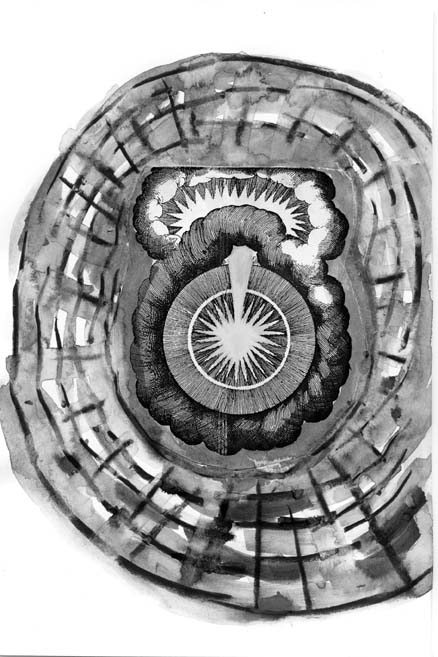
\includegraphics[width=100mm]{./imgs/caparc4.JPG}  
  %\hfill
\end{adjustwidth}

\end{figure}
\end{vplace}

\end{absolutelynopagebreak}

\pagebreak

\textbf{Luz}
\addcontentsline{toc}{chapter}{\textbf{Luz}\\ Lido por Régis Bonvicino}

Lido por Régis Bonvicino

\begin{verse}
Sucateiro rastafari\\
sentado na mureta, cabeça baixa\\
sob as palmeiras do largo\\
pés na mochila, garrafas pet\\[5pt]
\emph{player} do ecossistema global\\
um rato entra no bueiro.\\
O relógio da Luz\\
sob um sol de rachar\\[5pt]
daqui é apenas uma torre\\
o vapor sobe do asfalto.\\
Cicatriz na cara da puta\\
pista dupla, atravessa a avenida\\[5pt]
\emph{short} verde, blusa regata\\
cabelo curto, o michê esfria\\
os muros exalam um cheiro de urina.\\
A noite abate o dia\\[5pt]
um cachorro fareja, tranquilo,\\
a calçada limpa,\\
outro, órfão de um noia,\\
uiva na esquina.
\end{verse}

\pagebreak

\begin{absolutelynopagebreak}
\textbf{Interlude}
\addcontentsline{toc}{chapter}{\textbf{Interlude (2)}\\ por Rodrigo Dário}

Por Rodrigo Dário

\thispagestyle{empty}

\begin{vplace}
\begin{figure}[H]
%\begin{adjustwidth}{-3.2cm}{}
  \centering
  \vspace*{4cm}
  %\hspace{-0.5cm}
  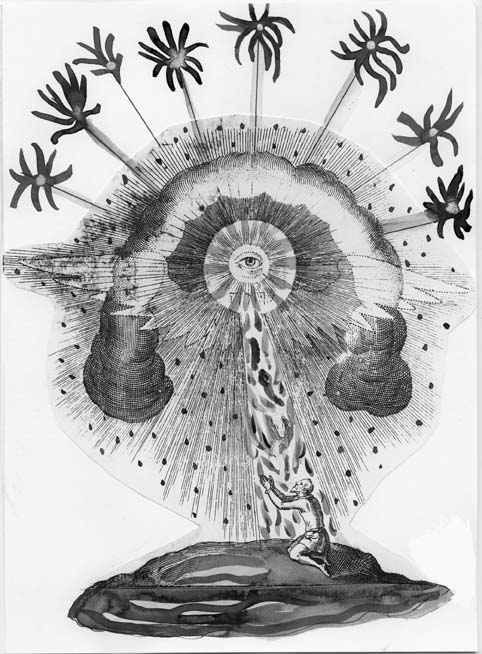
\includegraphics[width=100mm]{./imgs/caparc5.JPG}  
  %\hfill
%\end{adjustwidth}

\end{figure}
\end{vplace}

\end{absolutelynopagebreak}

\pagebreak

\begin{absolutelynopagebreak}
\textbf{Vinheta 4:}
\addcontentsline{toc}{chapter}{\textbf{Vinheta (4)}}

Hic Jacet Lepus

\thispagestyle{empty}

\begin{vplace}
\begin{figure}[H]
\begin{adjustwidth}{7.8cm}{}
  %\centering
  \vspace*{14.1cm}
  %\hspace{-0.5cm}
  \includegraphics[width=100mm]{./lebre.pdf}  
  %\hfill
\end{adjustwidth}

\end{figure}
\end{vplace}

\end{absolutelynopagebreak}

\pagebreak

\textbf{\emph{Hic Jacet Lepus}}
\addcontentsline{toc}{chapter}{\textbf{Hic Jacet Lepus}\\ Lido por Régis Bonvicino}

Lido por Régis Bonvicino

\begin{verse}
Perto de uma sinagoga, enquanto\\
o faxineiro varre a entrada do prédio,\\\
um catador, velho, de barba rala,\\
pega uma latrina na caçamba\\[5pt]
Outro catador, boné branco,\\
``ulalá'' grafado em azul acima da aba,\\
dois dentes podres à vista,\\
repete em voz alta: ``o lixo é sujo''\\[5pt]
Na banca, uma tevê: ataques na Síria\\
bombas na cara dos civis\\
Outro sucateiro, de mãe talvez zíngara,\\
saco plástico preto, aberto, percorre a calçada\\[5pt]
latas vazias de Pepsi, Coca, cerveja\\
pede na lanchonete, no \emph{self-service}, no bistrô\\
Na saída do \emph{shopping} militantes coletam assinaturas para\\
um manifesto em favor das abelhas,\\[5pt]
ágora na hora da xepa,\\
um santinho da Virgem colado no poste\\
um garoto negro, quase no ponto de ônibus,\\
um par de baseados no bolso,\\[5pt]
é preso em flagrante, por tráfico?\\
leva porrada na rua, \emph{ora pro nobis}\\
camburão, algemas\\
deus devolve o revólver
\end{verse}

\pagebreak

\textbf{A nova utopia (2)}
\addcontentsline{toc}{chapter}{\textbf{A nova utopia (2)}\\ Lido por Régis Bonvicino}

Lido por Régis Bonvicino

\begin{verse}
É um discurso estritamente atrelado à realidade\\
É um inferno fiscal\\
É uma empresa real\\
É o lado útil da palavra\\[5pt]
É uma brancaiada tola\\
É a nota mínima\\
É o aplicativo \emph{Equitable}\\
É um café da manhã sem lactose\\[5pt]
É a cerveja sem álcool e o cigarro eletrônico\\
É uma \emph{prece}, e não a Ave Maria, sussurrada\\
num beco de uma favela\\
É um sinônimo de vândalo\\[5pt]
É o alarme contra\\
o impacto ambiental de um passeio de barco\\
É um protesto contra aulas de inglês\\
É uma tr@b@lh@dor@ em transição de empregos\\[5pt]
É um supervilão asfixiando apenas machos\\
É um chá com escritores do \emph{website} e do jornal\\
É um \emph{pet} sem sobrepeso\\
É a queda programada da taxa de juros\\[5pt]
É um ladrão de galinhas\\
É um desvio de verbas públicas\\
É a vítima de um assalto\\
se desculpando com o assaltante\\[5pt]
É a redenção ecológica do joio\\
É um \emph{approach} jurídico para o diabo\\
É um cego paraolímpico\\
É um antiverso altamente subversivo\\[5pt]
É um alvo potencial do terrorismo linguístico\\
É um drácula \emph{hard-core} doando sangue\\
É o direito à segunda via garantido\\
É um morador de rua revirando uma lata de lixo seletivo\\[5pt]

\pagebreak

É o produto da venda legal de armas\\
Violinos afinam a brisa fétida\\
É uma lavagem de palavras\\
É uma filha convicta da pátria
\end{verse}

\pagebreak

\textbf{Áudio}
\addcontentsline{toc}{chapter}{\textbf{Áudio}\\ Lido por Caroline De Comi}

Lido por Caroline De Comi

\begin{verse}
O sol da manhã bate em sua cara\\
deitada no chão\\
rente à mureta do parque\\
fios de cabelo branco escapam da tiara\\[5pt]
cabeça sobre a bolsa\\
em frente à torre do relógio da estação\\
hibiscos vermelhos:\\
renques ao longo das grades\\[5pt]
mão sobre o rosto\\
talvez ela tenha chegado no último trem da noite\\
talvez ela não esteja dormindo\\
talvez ela esteja sem clientes\\[5pt]
vestido longo cinza\\
sapatos baixos, pele seca dos pés\\
talvez ela esteja a caminho do emprego\\
talvez ela vá pegar o metrô\\[5pt]
a polícia aqui não mata todos os dias\\
ao fundo palmeiras em linha\\
mendigo negro, cabeça baixa,\\
de novo, sentado na guia\\[5pt]
um ambulante vende água\\
talvez ela tenha escrito os versos:\\
``desatenta, fui castigada,\\
passei a vida ao largo''.\\[5pt]
talvez ela tenha feito algum dinheiro\\
talvez ela seja figurante de um filme\\
talvez ela seja um cartaz perdido\\
a luz, rasante, incide sobre as rugas de seu rosto\\[5pt]
a mandíbula de uma arara\\
um gavião pousa no topo de um cedro\\
mais alto que os prédios\\
talvez ela seja um acará ou uma carpa\\[5pt]

\pagebreak

espelhos d'água\\
uma andorinha, fosforescente, sobrevoa a grade\\
talvez ela não seja mais que um efeito de arte\\
talvez ela não passe de um \emph{close-up}
\end{verse}

\pagebreak

\textbf{Da janela do quarto}
\addcontentsline{toc}{chapter}{\textbf{Da janela do quarto}\\ Lido por Régis Bonvicino}

Lido por Régis Bonvicino

\begin{verse}
Manhã, janela do quarto do hotel:\\
o carroceiro puxa a carroça\\
uma van da Transcootour passa\\
pés descalços no asfalto\\[5pt]
gaivotas e urubus\\
se encaram por lixo, peixes e céu\\
banhistas em sua rotina mecânica de\\
sol, areia e ginástica\\[5pt]
duas putas insones roçam\\
os peitos nos vidros\\
de um Honda Civic.\\
A garota de Ipanema\\[5pt]
de Vinícius e Tom Jobim\\
mora hoje em Arrelia, Andaraí\\
é mais que um poema\\
paga o dízimo, da igreja e da milícia,\\[5pt]
ônibus lotado, caindo aos pedaços,\\
de moto, um PM arranca o celular\\
hoje pelo menos faltou presunto\\
a caminho do mar,\\[5pt]
e sua irmã gêmea, a coisa mais linda,\\
mora com o gigolô da boca\\
em Drummond, Cachambi\\
Papelotes de cristal e cocaína no sutiã\\[5pt]
à noite, frequenta o Leblon\\
Troca de tiros na \emph{web} e na tevê\\
Complexo da Maré,\\
Bossa Nova \emph{nightmare}
\end{verse}


\pagebreak

\textbf{\emph{The new utopia} (1)}
\addcontentsline{toc}{chapter}{\textbf{\emph{The new utopia (1)}}\\Translated by Odile Cisneros\\ Lido por Charles Bersntein}

Translated by Odile Cisneros

Lido por Charles Bersntein

\bigskip

The new utopia is a black butterfly, inattentive, with lush eyes. The
new utopia is in favor of the ruthless protection of animals. The new
utopia is inclusionary, participatory. The new utopia is a tuned chorus
of discontent. Is a burly ex guerrilla, a government strongman. The new
utopia has insider information available. It is an ex leprosy patient.
The new utopia rejects the figure of Our Lady masturbating. The new
utopia fights for the rights of sex work service providers. The new
utopia shares, in moderation, materialistic ideals. The new utopia dies
standing. It sells both duty-free items and financial detox. The new
utopia is our civic duty. The new utopia praises corporate
sustainability. The new utopia knows you can be an Arab and a Muslim, an
Arab and not a Muslim, a Muslim and not an Arab. You can be Black
without being White, White without being Black. The new utopia is
\emph{Le Monde's} freedom of expression enshrined forever. The new
utopia is a reckoning against the obscurantism of others. The new utopia
rejects politically expedient factoids. The new utopia is a bit Shiite,
only when strictly unavoidable. Is an American tourist visiting the Abu
Ghraib Museum. The new utopia has logos and slogans. Denounces killings
in poor neighborhoods. The new utopia condemns actions, circulates
petitions; it champions graffiti; the new utopia advocates bikes. The
new utopia is unconditional respect for underachievers. Condemns corrupt
leaders. Is an ex crook. It uses its own dictionary. Looks before it
leaps. Rejects words and calls for action. The new utopia is an ex
amputee. Is an open wing in flight. Is a showroom of natural lushness.
Is a sky with dark clouds under control. Is a bookcase in a bathroom. Is
the widow of Jorge Luis Borges explaining his creative process. The new
utopia is an ex \emph{macumba} devotee, an ex drunk, an ex \emph{Exu}
punk. Is a whitie with a Black soul. The new utopia is also the
torch-bearing Native politicking daily on social networks. The new
utopia is an ex beautician with nail extensions. Is a trans spy catching
some sun on a router. Is an ex savage. Is an ex bitch. Is an ex hustler.
Is a lesbian. Is an ex pariah. Is a myriad of prize-winning poet
franchises. Is a poem in tune with the times.

\pagebreak

\textbf{A nova utopia (7)}
\addcontentsline{toc}{chapter}{\textbf{A nova utopia (7)}\\ Lido por Caroline De Comi
\medskip}

Lido por Caroline De Comi

\bigskip

\emph{To dream has been the business of my life.}~A nova utopia~mata por
adição e, entre outras coisas, por agonismo opioide. Faz seu inimigo
sentir náuseas, sonolência, vertigem, vômitos, dor de cabeça, pressão
baixa e choque. Faz seu inimigo falar com voz de lixa: ela não brinca em
serviço. A nova utopia não é um despropósito.~O novo utopista não é um
dândi da sombra. É o drone suicida roubado da Kalashnikov: carrega
explosivos e~abre caminhos na selva, na favela, nas cidades. Tudo pela
causa. Também ecológica, é a favor de cocaína batizada com pó de
nenúfar. É a favor, unicamente, de obras como as de Shakespeare a cada
manhã. A nova utopia -- mirando um futuro melhor -- faz tráfico limpo. O
raio de sol só aparece à noite, para desanuviar. Pense, pense, você está
na Terra: não há remédio. Fique tranquila, numa boa. Tantos miligramas
de Depakote, tantos de Topiramato, a bula do Aristab -- a rotina diária
sem tréguas de pílulas por uma década. Comece por Zyprexa. Um robô morre
em Marte. Um cara atira, entre prateleiras, contra a própria cabeça
dentro da farmácia. Nada, absolutamente nada, mais um saco de merda sem
qualquer mérito.~Má notícia não existe.~Dinheiro não fede.~A chuva, a
chuva, a tempestade, uma enxurrada de lixo sobe dos bueiros às ruas. Sob
a marquise, um bispo se esgoela num megafone: ``botar um baseado nos
lábios é como fazer sexo oral para o diabo''. Só pode ser o trecho de um
filme, ouça o refrão da música: ``eles disseram que o inferno ferve''.~O
novo utopista é um sicário \emph{indie}. É chefe e servo de si mesmo. É
uma fera. Atira de bate-pronto nos sequestradores de cérebros e nos
revendedores de memória, que operam o mercado negro. Mata de verdade.~É
a favor do \emph{copyright}. É contra o \emph{copyleft}. O novo utopista
aplica doses pesadas de morfina nos algoritmos. Para ele, o algoritmo
atropela o trabalho. Outra cena? \emph{Crack} é a vitória. Um mendigo
puxa uma pedra na lata amassada de Coca-Cola. O novo utopista batalha
pela liberdade entre muros. Pede a benção à deusa~guarani Jururá-Açú
para assassinar o diabo do velho utopista.~À semelhança dela, entra e
sai do inferno como quem troca de camisa.~Não faz papel de morto
coadjuvante.~O ódio move mais do que qualquer programa político.~Só pode
ser mesmo um filme. Olhe o décor.~Trabalha também com~fungos
alucinógenos e LSD, para fazer mais grana para a luta.~É um ponto de
partida. Por que dizer isto aqui? Cai o letreiro: tantos miligramas de
Quetiapina, o antipsicótico atípico,~as bulas, o Latuda: para que
desespero? Johnson \& Johnson, Pfizer, Merck \& Co, Bayer, Novartis, EMS
Corp, Roche holding, Libra. Um grito talvez em \emph{off} se ouça no
cenário. Uma garota se joga do topo do edifício. Sonhar, sonhar, sonhar,
é o grande negócio da vida!

\chapter{Participantes do álbum}

\section{Rodrigo Dário}

Nascido em São Paulo em 1982, faz e produz música
desde 2006, sua principal atividade artística, ao lado do
desenho. É membro fundador e artista sonoro atuante dos
selos musicais Al Revés e De Lírio Records. Já apresentou
seus trabalhos em eventos como Hypersônica (\versal{FILE}), \versal{SIM}
São Paulo, 30ª Bienal de \versal{SP}, Improvise!, Festival Música
Estranha, entre outros. Trabalha com música eletrônica,
experimentos sonoros, livre improviso, colagem sonora
e fieldrecording. Em 2014, algumas de suas composições
fizeram da trilha sonora parte do filme \emph{A misteriosa morte
de Pérola} (Demência, Cerberus e Curvas). Atualmente
também integra os projetos Acauã e Beat Brasilis Orquestra.

Já se apresentou ao lado de: \versal{SPIO} Orquestra (2018), Al Revés
(2006 a 2018), Otomo Yoshihide e Loop B (2018, na Redbull
Station no evento Improfest), performances de arte"-sonora,
ruido e improviso livre no evento Campos de Experimentação
Sonora em \versal{SJC}: com Agnes Havizdalek, Alexandre Marino
e Bruno Hiss (julho de 2017); Dissonance From Hell *\versal{NO
FEST}* no Centro Cultural Zapata (junho 2017); \versal{IMPROVISE!}
na Trackers (residente do evento de 2017 a 2018); Silver Tape
no Estúdio Fitacrepe SP -- Ateliê de som e movimento (abril
de 2017); Estúdio Fitacrepe \versal{SP} -- Ateliê de som e movimento:
com Bruno Hiss, Alexandre Marino, Leandro Archela e Felipe
Vilasanchez (março de 2017); \versal{XIII ENCUN -- MIS} Campinas/\versal{SP}:
com Bruno Hiss e Alexandre Marino (dezembro de 2015);
Audio Rebel/\versal{RJ} (novembro de 2015); Ibrasotope Música
Experimental (outrubro de 2015); Intervalos Musicais -- 10
anos de \versal{EACH}, Escola de Artes, Ciências e Humanidades,
Universidade de São Paulo -- Campus Leste: com Alexandre
Marino e Bruno Hiss (agosto de 2015); Performance de arte"-sonora
e ruído em ``Ressonância'', show de rádio de Alexandre
Marino e Rodrigo Dário, apresentado por Leandro Nerefuh, na
web"-rádio Tatu no ar, Centro Cultural São Paulo (novembro
de 2014); Espaço Cultural Walden, São Paulo: (dezembro
de 2014); Encontros Abertos Intermeios, Intermeios Casa de
Arte e Livros, São Paulo: com Vitor Kisil Miskalo, Magno
Caligman, Amphis \& eue (maio de 2014); com Amphis, eue
\& Uessels (abril de 2014); Mobile"-radio (mobile"-radio.net),
de Sarah Washington \& Knut Aufermann, na 30ª Bienal de
Arte de São Paulo (outubro de 2013); solo Politicica (setembro
de 2013); com Border Pigs (Bruno Hiss, Rafael Gherini e
Alexandre Marino) (1º setembro de 2013); Coletivo Al Revés
Ao Vivo. Hipersônica -- \versal{FILE} (Festival Internacional de
Linguagem Eletrônica). Teatro da \versal{FIESP}, São Paulo (agosto de
2006). \enlargethispage{\textheight}

Websites sonoros: \emph{soundcloud.com/d\_rw}, \emph{soundcloud.com/rodrigodario} e \emph{deliriorecords.bandcamp.com}. 

\pagebreak

\section{Caroline De Comi}

Nascida em São Paulo, soprano coloratura atuante não apenas no
repertório operístico, como na música de câmara e contemporânea,
Caroline De Comi é uma das mais versáteis cantoras líricas brasileiras
da nova geração.

Dentre seus trabalhos mais recentes está Rainha da Noite, na ópera
\emph{A flauta mágica} de W. A. Mozart, no Teatro Municipal de Santiago
do Chile, e Marzelline, na ópera \emph{Fidelio} de Beethoven, no Theatro
Municipal de São Paulo. Atuou em montagens de ópera no Teatro Municipal
de São Paulo, como \emph{O rouxinol} de Stravinsky (no papel título) e
na premiadíssima \emph{L'enfant et les sortilèges}, de Ravel (como o
Fogo, a Princesa e o Rouxinol). Participou de óperas como
\emph{Rigoletto} (Gilda), \emph{Fidelio} (Marzelline), \emph{Lucia de
Lammermoor} (Lucia), \emph{Der Schauspieldirektor} (Madame Herz),
\emph{Il Matrimonio Segreto} (como Elisetta), \emph{La Traviatta}
(Violeta), \emph{Don Pasquale} (Norina), \emph{O barbeiro de Sevilha}
(Berta e Rosina), \emph{La Serva Padrona} (Serpina) e na estreia da
também premiada \emph{O menino e a liberdade} (como ``a moça''), de
Ronaldo Miranda. Esteve sob a direção de Myriam Singer, Lívia Sabag,
Mauro Wrona, João Malatian, Alvize Camozzi, Regina Galdino, Marcia
Milhazes e Cleber Papa. Integrando a Companhia Ópera Curta, realizou
diversas récitas como Rosina, em \emph{O barbeiro de Sevilha}, e como
Violetta, em \emph{La Traviatta}. Em 2010, foi eleita pelo \emph{blog
Ópera e Ballet} destaque lírico do ano por sua atuação como Gilda, no
\emph{Rigoletto} de G. Verdi, no Teatro São Pedro. Foi solista em obras
de concerto como \emph{Stabat Mater} de G. B. Pergolesi, \emph{A
criação} de Haydn (como Eva), na \emph{Missa da Coroação} e
\emph{Exsultate Jubilate} de W. A. Mozart, \emph{Oratório Ester} de
Antonio Leal Moreira (Ester e Harbona), \emph{Missa em sol maior} de F.
Schubert, \emph{Requiem} de G. Fauré, \emph{Oratório de Natal} de
Saint"-Saëns, no \emph{Messias} de Haendel, \emph{Les Illuminations} de
Britten, \emph{Tragédie de Salomé} de Florent Schmitt e na estreia da
obra \emph{Cantata para Caroline} de Maurício De Bonis. Apresentou"-se à
frente da Orquestra Sinfônica do Estado de São Paulo (Osesp), da
Orquestra Experimental de Repertório (\versal{OER}), da Orquestra Acadêmica de
São Paulo, da Orquestra de Câmara da \versal{USP}, da Orquestra Sinfônica da \versal{USP},
do Coro da Osesp e da Orquestra Municipal de Jundiaí. Atuou sob a
regência de Roberto Minczuk, Jamil Maluf, Cláudio Cruz, José Luis
Domínguez, Yan Pascal Tortelier, John Neschling, Roberto Duarte, Gabriel
Rhein Schirato, Emiliano Patarra, Carlos Moreno, Claudia Feres, Jack
Fortner, Naomi Munakata, Luciano Camargo, entre outros. Foi solista em
algumas das principais salas de concerto do país, como o Theatro
Municipal de São Paulo, a Sala São Paulo, o Theatro São Pedro, o Teatro
Arthur Rubinstein, Auditório Cláudio Santoro (em Campos do Jordão), o
auditório da \versal{CPFL} Cultura (em Campinas), a Sala Cecília Meireles (no Rio
de Janeiro), o Teatro Nacional Cláudio Santoro (em Brasília), além da
Embaixada do Brasil em Assunção, no Paraguai. Recentemente esteve em
turnê por diversas cidades dos Estados Unidos, como Riverside, Santa
Clara, Baton Rouge e Philadelphia.

Graduou"-se em
Canto e Arte Lírica pela \versal{ECA-USP}, onde iniciou seu estudo de canto com o
tenor Benito Maresca. Tendo Isabel Maresca como sua principal
orientadora vocal, frequentou também cursos e masterclasses no Brasil e
no exterior com Tamás Salgó, Niza de Castro Tank, Anna Korondi, Susan
Bullock, Christina Landshamer, Peter Schreier, Luisa Castellani, Ian
Storey e Eleonora Leonini.

Participou do ciclo de concertos ``Willy Manifesto'' (em homenagem aos
setenta anos de Willy Corrêa de Oliveira), da série Panorama da Música
Brasileira (Unicamp), da 39ª Bienal de Música Brasileira Contemporânea e
constantemente participa do Festival Música Nova de São Paulo.
Realizando estreias mundiais e tendo diversas obras dedicadas a ela, vem
se apresentando no Brasil e no exterior ao lado de respeitados músicos
brasileiros como Maurício De Bonis, Gilson Antunes e Joaquim Abreu.
Entre suas gravações estão o DVD \emph{A Flauta Mágica, o Maestro e a
Feiticeira} (Tucca), o \versal{CD} \emph{Willy Corrêa de Oliveira, o presente}
(ÁguaForte), o \versal{CD} \emph{Olivier Toni: Só Isso e Nada Mais} (Sesc) e o \versal{CD}
\emph{Festival Música Nova} (Sesc). \emph{Website}:
http://www.carolinedecomi.com/biografia.html.

\section{Charles Bernstein}

Foi o vencedor, na Universidade de Yale, do
\emph{Bollingen Prize for
American Poetry} de 2019. O \emph{Bollingen Prize}, criado por Paul
Mellon em 1949, é concedido bianualmente pela Biblioteca da Universidade
de Yale, através da Beinecke Rare Book and Manuscript Library, a um
poeta americano.

Bernstein é o 51º poeta a ser honrado com o prêmio e
soma"-se à lista de vencedores, que inclui Ezra Pound, W.H. Auden,
Marianne Moore, Wallace Stevens, Robert Frost, E.E. Cummings, John
Ashbery, Robert Creeley, Glück, Charles Wright, Gary Snyder e outros.

``Como poeta, editor, crítico, tradutor e educador, a dedicação de
décadas de Charles Bernstein à comunidade das artes e letras reflete a
profunda compreensão que ele tem da importância da língua na formação da
cultura em todos os campos de empreendimentos.'' Essa foi a opinião dos
três membros do comitê que julgou a concessão do prêmio.

\begin{quote}
Sua extraordinária nova coletânea de poemas \emph{Near/Miss} mostra um
Bernstein que, com sua sátira tipicamente incisiva e sua agudeza de
espírito, sabe desmontar os lugares"-comuns que norteiam os diversos
discursos públicos. Contudo, em momentos de pena intensa, a obra atinge
as profundezas onde o poeta público deve saber encontrar palavras para o
sofrimento individual. Sua obra interroga incessantemente, como que
palavra por palavra, a língua e sua natureza performática.
\end{quote}

Bernstein é autor de numerosos livros de poesia, como \emph{Near/Miss},
\emph{Recalculating} e \emph{All the Whiskey in Heaven: Selected Poems},
entre muitos outros. Sua coleção de ensaios inclui \emph{Pitch of
Poetry}, \emph{Attack of the Difficult Poems: Essays and Inventions} e
\emph{A Poetics}. Bernstein também é conhecido por suas traduções,
colaborações com artistas e libretos. Com Al Filreis, é o cofundador do
\emph{Penn Sound}, um arquivo extenso de poesia gravada. Bernstein foi
eleito Membro da \emph{American Academy of Arts \& Sciences}, em 2006.
Outros prêmios e reconhecimentos incluem o \emph{Janus Pannonius Grand
Prize for Poetry}, o \emph{Münster Prize for International Poetry}; uma
bolsa de pesquisa do \emph{John Simon} \emph{Guggenheim Memorial}; e uma
dotação do \emph{National Endowment for the Arts Creative
Writing.} Bernstein foi professor de Inglês e de Literatura Comparada de
Donald T. Regan na Universidade da Pennsylvania.

Os juízes -- Ange Mlinko, Claudia Rankine, e Evie Shockley -- assim se
manifestaram: ``Ao longo de sua carreira, Bernstein tem promovido um
diálogo vibrante entre tendências líricas e antilíricas, nas tradições
poéticas que herdamos; com isso ele deu forma e questionou, definiu e
desmontou ideias e suposições, revelando as mais amplas e mais profundas
competências da poesia.''

``A poesia americana contemporânea prospera em sua pequena escala por
entre diferenças de forma radicais'' -- diz Bernstein. ``Sua liberdade
está fundamentada nas várias abordagens dos que a praticam e em sua
resistência à popularidade orientada para o mercado. A invenção poética
é tão fundamental para nossa democracia como a Carta de Direitos -- algo
a ser celebrado com exuberância e prazer.''

``Estamos emocionados com o fato de que os juízes do \emph{Bollingen
Prize} de 2019 tenham escolhido Charles Bernstein, um poeta cuja obra
criativa e crítica tem revivescido a poesia e a poética americana'',
observou Kuhl. ``Os poemas de seu último livro, \emph{Near/Miss},
exploram a própria natureza da poesia.''

\section{Régis Bonvicino}

Nascido em São Paulo em 1955, Régis Bonvicino reuniu seus poemas numa
publicação em \emph{Até agora: poemas reunidos} (São Paulo: Imprensa
Oficial, 2010) e numa seleção, traduzida para o inglês e publicada em
2017 (\emph{Beyond the Wall: New Selected Poems}. Los Angeles: Green
Integer). Ele faz parte de uma geração de poetas brasileiros que surgiu
com o declínio da Poesia Concreta e sob os ecos do Tropicalismo na
década de 1970.

Como habitante de uma São Paulo global, a poesia de Bonvicino reflete
igualmente a condição precária dos seres urbanos contemporâneos nessas
décadas. Embora tenha recebido apenas um prêmio em seu país, Bonvicino é
um dos poucos poetas brasileiros contemporâneos cujo trabalho tem sido
significativamente traduzido e publicado no estrangeiro, o que é prova
de sua reputação internacional. Como diz o poeta francês Michel
Delville:

\begin{quote}
{[}\ldots{}{]} a poesia de Bonvicino consegue sua intensidade
extraordinária da atenção renovada que ele dá ao ato de olhar, em si, da
contemplação de relações e oposições e do desejo de alargar a imaginação
seguindo linhas de disjunção, de extensão, de regeneração. Régis
Bonvicino é certamente um dos poetas mais desafiadores e interessantes
dos últimos vinte e cinco anos.
\end{quote}

Filho de Alva Flôr Ferreira de Oliveira e de Odayr Rodrigues Bonvicino,
Régis Rodrigues Bonvicino nasceu em São Paulo em 25 de fevereiro do ano
já mencionado de 1955. Frequentou o curso primário da Escola Nossa
Senhora das Graças e o secundário no Colégio Santa Cruz. Ele mesmo
lembra da liberdade com que se podia jogar futebol nas ruas e perambular
pelos vários bairros de uma São Paulo ``grande e, mesmo assim,
civilizada''. Bonvicino cursou a Faculdade de Direito da \versal{USP}, onde se
formou em 1978.

No que se refere ao cinema, central para este autor, admira e tem como
inspirador, desde a juventude, o Neorrealismo italiano, incluindo
Roberto Rossellini, Federico Fellini, Michelangelo Antonioni, Pier Paolo
Pasolini e Vittorio De Sica, entre tantos outros. De seus ícones
literários, Bonvicino lembra haver recortado o obituário de Ezra Pound,
de um jornal de 1972. Lia e apreciava Álvares de Azevedo, Carlos
Drummond de Andrade, Fernando Pessoa, Mário de Sá Carneiro e João Cabral
de Melo Neto, mas seu poeta favorito era Cesário Verde.

Sua estreia literária deu"-se em 1975, no \emph{Jornal do Arena}. Começou
trabalhando como colunista em jornais e revistas de São Paulo, tais como
\emph{Jornal da Tarde}, \emph{Isto É}, \emph{Folha de S.Paulo}, até
1989. Começou muito cedo a se interessar por poesia, fundando a revista
\emph{Poesiaem G}, em meados da década de 1970. A ela se seguiu outra
revista inovadora, porém efêmera: \emph{Qorpo Estranho}, cujos dois
números Bonvicino coeditou com o artista espanhol Julio Plaza. Essas
pequenas revistas foram fundamentais para proporcionar espaço a três
gerações de poetas excluídos dos suplementos culturais dos principais
jornais, tais como o \emph{Jornal do Brasil} e \emph{O Estado de S.
Paulo}, durante a ditadura.

Bonvicino autoeditou seu primeiro livro de poemas, \emph{Bicho papel}
(1975), numa publicação modesta de trezentos exemplares. Outra
autoedição apareceu pouco depois, em 1978, \emph{Régis Hotel}. Numa
resenha a respeito de \emph{Régis Hotel} (\emph{Polo Cultural},
Curitiba, 18 de maio de 1978), Paulo Leminski notou que os primeiros
poemas de Bonvicino, como, por exemplo, ``?avolho'', deixavam entrever
uma espécie de ``filiação perplexa ao concretismo''. Numa manipulação
feita com a palavra \emph{lavolho}, marca de gotas para os olhos, no
Brasil, o poema cutucava tanto a linguagem da propaganda quanto a ênfase
da poesia concreta na cultura visual e de massa.

Em 1979, casou"-se e desse casamento teve dois filhos: João Rodrigues da
Costa Bonvicino, nascido em 1979, e Marcelo Flores Rodrigues da Costa
Bonvicino, nascido em 1987. Um evento traumático na vida de Bonvicino,
nesse período, foi o suicídio de sua mãe, Alva Flôr, em abril 1979. Em
1975, Bonvicino iniciou uma amizade também epistolar com Paulo Leminski,
que morava em Curitiba. Leminski teve papel decisivo na busca de
Bonvicino por modelos poéticos outros que a poesia concreta, e
vice"-versa, num diálogo fértil, embora divergissem em vários aspectos.

Na década de 1980, Bonvicino lançou (em colaboração com a artista Regina
Silveira e Julio Plaza) \emph{Do Grapefruit} (1981), um livro de Yoko
Ono com traduções feitas por Bonvicino e trabalhos de arte de Silveira e
Plaza. Bonvicino transformou as instruções conceituais em poemas. Em
seguida, ele escreveu prefácios para catálogos de artes plásticas,
incluindo um para o argentino León Ferrari (1989). Nesse período, foi
conselheiro parlamentar em Brasília, durante a Assembleia Constituinte
de 1987 a 1988.

O livro seguinte de Bonvicino, \emph{Sósia da cópia}, saiu em 1983. Tal
obra contém também um importante poema autobiográfico, ``vida, paixão e
praga de rb'', em que Sebastião Uchoa Leite viu um ``retrato da
autoflagelação do poeta como diluidor (no sentido poundiano)'' e
sobretudo uma provocação, em sua caracterização do ``poeta como uma
`mera maldição', o imitador de imitações'' (\emph{Leia Livros}, junho de
1983). Leminski viu o livro como ``uma discussão viva e criativa do
próprio conceito de originalidade'' (Revista \emph{Veja}, 13 de julho de
1983). Entre os autores assimilados e traduzidos, um que desperta o
interesse especial de Bonvicino foi o simbolista francês Jules Laforgue,
cujos trabalhos traduziu e publicou em 1989, no livro \emph{Litanias da
lua}, que inaugurou sua contribuição como tradutor de poesia.

Em 1984 Bonvicino também editou e publicou \emph{Desbragada}, uma
antologia da obra do poeta experimental e visual Edgard Braga, cuja
poesia caligráfica ele admirava por sua espontaneidade e singularidade.

\emph{Sósia da cópia}, por seu caráter crítico, já aponta para o que
será a obra de Bonvicino da fase seguinte. \emph{Más companhias} (1987)
foi definido pelo autor como ``um livro explosivo com poemas muito
intensos que causaram um pequeno escândalo''. Trata-se de um volume
esguio, sem numeração de páginas, que explora a questão da autoria a
partir de peças de poetas como Borges, Gregory Corso, Safo e Edward
Lear. A dicção do livro é bruta, direta. Publicado em 1990, \emph{33
poemas} revela o surgimento da rima assonante como um dos fatores de
estruturação dos poemas. Os poemas concentram"-se mais na observação do
mundo da natureza, mas -- mesmo assim -- a cidade continua muito
presente, de diferentes e inesperadas maneiras. \emph{33 poemas}
entretém um diálogo com a ambiência em que os objetos alteram o ser dos
sujeitos no mundo. Tal livro deu a Bonvicino o Prêmio Jabuti de 1991.

Em 1990, Bonvicino tornou"-se magistrado por concurso. Em 1992, ele se
casou com a psicanalista Darly Menconi, com quem teve dois filhos: Bruna
Menconi Bonvicino (que, em razão de bipolaridade grave, se suicida em 19
de outubro de 2018), nascida em 1992, e Felipe Menconi Bonvicino,
nascido em 2010. Em 1992, publicou \emph{Uma carta uma brasa através:
cartas a Régis Bonvicino, 1976-1981}, uma reunião das cartas que recebeu
de Leminski. As cartas que ele escreveu a Leminski não foram
preservadas, logo não constam da publicação; porém, numa edição
subsequente, foram acrescentados material crítico e uma introdução
atualizada do próprio Bonvicino. Nessa época, Leminski não fazia o
sucesso que faz hoje.

A partir de 1990, Bonvicino passou a ser conhecido internacionalmente
graças à participação em leituras de poemas, especialmente em Buenos
Aires (1990), na Feira de Livros de Miami (1992), e em Copenhagen
(1993). Em 1995, por ocasião de uma viagem à França, participou da
Terceira Bienal Internacional de Poetas em Val"-de"-Marne, e leu seus
poemas em Paris (Maison de l'Amérique Latine) e em Marselha
(International Poetry Center).

O livro seguinte de Bonvicino, \emph{Outros poemas} (1983), evita o
\emph{layout} não tradicional, um abandono de poucas experiências
visuais dos primeiros tempos. Numa entrevista a \emph{Caracol"-Viola 43}
(1998), Bonvicino caracterizou essa escolha como sendo uma alternativa à
oposição binária entre poesia visual e verso tradicional:

\begin{quote}
Eu não gosto dos experimentos de poesia visual que são feitos hoje.
Trinta ou quarenta anos atrás um poema visual tinha o sentido de
ruptura. Hoje não passa da imitação de um anúncio. Não tem mais o papel
de crítica {[}\ldots{}{]}. Contudo, também não gosto da ideia de a
``linha de verso'' ser uma unidade da poesia -- não da minha, de
qualquer modo. A saída do ``verso'' (tradicional) não é necessariamente
a poesia visual {[}\ldots{}{]}. Eu escrevo em versos, mas sem me
importar com o metro ou com o verso branco, mas sim prestando atenção
aos ritmos da respiração ou do sistema nervoso, por exemplo.
\end{quote}

Em meados da década de 1990, Bonvicino publicou, em parceria com Guto
Lacaz, um livro infantil dedicado aos filhos, \emph{Num zoológico de
letras} (1994). Também voltou a lançar seus primeiros trabalhos num
único volume, \emph{Primeiro tempo: reunindo os livros Sósia da cópia,
Régis Hotel e Bicho papel} (1995), e realizou uma tradução do poeta
vanguardista argentino Oliverio Girondo, \emph{A pupila do zero = En la
masmédula} (1995). A primeira em todo o mundo deste grande poeta
portenho.

Em \emph{Ossos de borboletas} (1996), o humor é muito mais contemplativo
e menos lúdico do que nos primeiros trabalhos. O diálogo com o poeta
americano Robert Creeley nota"-se nos versos curtos, especificamente em
``Março (2)'', um poema minimalista que lida com diferenças e oposições
básicas, e em outros breves esboços urbanos. A crítica norte"-americana
Marjorie Perloff afirmou sobre este volume:

\begin{quote}
As novas líricas de Bonvicino, econômicas, minimais, tensas e
brilhantemente articuladas, lembram a cada instante a diferença que
podem fazer os ``ossos de borboletas'' {[}\ldots{}{]} e ele também sabe,
ao medir"-se com uma ``escola'' com mestres americanos do calibre de
William Carlos William, Robert Creeley, George Oppen -- que
{[}\ldots{}{]} as pequenas palavras -- \emph{entre}, \emph{como},
\emph{alguém} -- são tão importantes como suas pretensiosas primas, as
palavras que pretendem designar as grandes verdades acerca da
experiência\ldots{}
\end{quote}

Com efeito, por alguns anos, Bonvicino esteve realmente estudando os
poetas modernistas e contemporâneos da América do Norte, à procura de
novas perspectivas poéticas. Em 1996 esteve com Michael Palmer para uma
leitura de poemas na San Francisco State University. Nesse mesmo ano,
Bonvicino publicou em livros traduções de poemas de Palmer
(``Passagens''), de Robert Creeley (``Salve!''). Outro livro com poemas
de Creeley, \emph{A um: poemas = As one}, saiu em 1997, junto com uma
seleção de poemas de Guy Bennett, Charles Bernstein, Norma Cole e
Douglas Messerli intitulada \emph{Duetos: 4 poetas norte"-americanos
contemporâneos}. Nesse mesmo ano Bonvicino publicou também
\emph{Together 1996} (\emph{um poema: vozes}), um livro de poemas
\emph{renga} para o qual ele convidou 28 poetas a contribuírem com um
segmento.

O interesse de Bonvicino por manter um diálogo poético Norte/Sul incluía
também o esforço para disseminar a poesia brasileira nos Estados Unidos.
Com esse intuito, colaborou com Palmer para a publicação da antologia
\emph{Nothing the Sun Could Not Explain: 20 Contemporary Brazilian
Poets}, nos Estados Unidos, em 1997. O volume foi reeditado como
\emph{The \versal{PIP} Anthology of World Poetry of the 20th Century Volume 3},
em 2003. Essa era a primeira tentativa, desde Elisabeth Bishop, de expor
a um público não só americano, mas, mais especificamente, anglófono, uma
seleção de poetas brasileiros contemporâneos.

Em 1998, Bonvicino esteve presente na \emph{Segue Performance
Foundation} de Nova York, juntamente com Charles Bernstein, o poeta
experimentalista americano fundador do importante movimento
\emph{L=A=N=G=U=A=G=E}.

Em 1999, Bonvicino realizou leituras na Universidade de Santiago de
Compostela, na Espanha. O livro \emph{Me transformo ou O Filho de
Sêmele}, uma espécie de protesto contra a situação nos Balcãs, com
tradução em seis línguas, saiu também em 1998, impresso especialmente
para as leituras de Compostela.

O mesmo ano de 1999, no Brasil, foi muito produtivo para Bonvicino. Uma
segunda edição aumentada das cartas de Leminski a Bonvicino foi
realizada com o título \emph{Envie meu dicionário: cartas e alguma
crítica}. Bonvicino também publicou \emph{Primeiras palavras}, a
tradução de uma obra do poeta, dramaturgo e editor americano Douglas
Messerli. A editora de Messerli, Sun and Moon Press, que já não existe,
havia publicado as antologias de poesia brasileira realizadas por Régis,
e a editora que a sucedeu, Green Integer, publicou dois volumes de
poemas de Bonvicino em tradução inglesa. No ano de 1999 foi também
publicado \emph{Céu-eclipse}, o novo volume de poemas de Bonvicino que
Aurora Bernardini chamou de ``as predições (talvez) do novo milênio''
(\emph{Jornal da Tarde}, 4 de setembro de 1999), e que também ressaltou
o ``novo literalismo'' com que Bonvicino explorava ``desafios
filosóficos''. Em sua resenha, Wilson Bueno notava como Régis ``luta
numa direção que, generosamente, parecia indicar caminhos'', e
salientava a ``capacidade da língua para reordenar o mundo dentro de
nós'' e que ``o mundo muda de luz a sombra em mais um dia''
(\emph{Gazeta do Povo}, 29 de agosto de 1999).

Traduzido por Robert Creeley, Michael Palmer e outros, o primeiro livro
em inglês de Bonvicino, \emph{Sky-Eclipse; Selected Poems}, saiu no ano
2000. No ano seguinte foi publicado um volume multifacetado de
colaborações com Palmer, \emph{Cadenciando"-um"-ning, um samba, para o
outro: poemas, traduções, diálogos} (2001). O título do livro foi
retirado de um verso de um poema de Palmer em que ele ``relata'' a
visita que fez a São Paulo, em maio de 1997: ``o animal alfabeto/ deu
volta por cima/ com suas vinte e três asas/ cadenciando"-um"-ning, um
samba para o morto''. O poema sugeriu o motivo do samba a Bonvicino, que
entendeu o projeto não como uma ``tradução'', mas antes como um
``diálogo de riscos mútuos''. A atitude de Bonvicino de procurar
conexões fora do Brasil encontrou, muitas vezes, reações negativas em
seu país.

Como colunista, Bonvicino levou adiante suas contribuições para a
\emph{Folha de S.Paulo} e, em 2000, iniciou suas colaborações para
\emph{O Estado de S. Paulo}. Nesse ano realizou leituras de poemas em
Iowa City, junto com Michael Palmer, e em Chicago. Em maio de 2001 foi
para Coimbra, Portugal, para o \versal{IV} Encontro Internacional de Poetas, na
Universidade de Coimbra. No ano seguinte, foi publicada em Portugal uma
coletânea de seus poemas com o título de \emph{Lindero nuevo vedado:
antologia poética.}

Em 2000 Bonvicino fundou \emph{Sibila: Revista de Poesia e Crítica
Literária}, periódico que ele codirigiu com Charles Bernstein. Entre os
anos de 2001 e 2006, \emph{Sibila} publicou seus números impressos,
tornando"-se uma revista eletrônica e \emph{website} depois de 2007.

\emph{Hilo de piedra}, um livro com poemas de Bonvicino, foi traduzido
para o espanhol pela revista \emph{Sibila} de Sevilha (sem ligação com a
revista de Bonvicino). Os dois livros seguintes, \emph{Remorsos do
Cosmos} (\emph{de ter vindo ao sol}), de 2003, e \emph{Página Orfã}, de
2007, são coleções em que imagens e linguagem da mídia pós"-moderna e a
consciência das ameaças da globalização colidem com as descrições da
crua realidade da vida urbana. Alcir Pécora viu ``um cosmo em estado de
calamidade belicosa {[}\ldots{}{]} persecutório {[}\ldots{}{]} insone
{[}\ldots{}{]} limitado por fronteiras rígidas e opressivas'' (``Caderno
Mais!'', \emph{Folha de S.Paulo}, janeiro de 2004). A técnica de
montagem de \emph{Página órfã} junta peças da sucata e dos depósitos de
lixo da língua para expor a violência local e global. Alcides Villaça
viu nela ecos de um ``vitalismo que impressiona, no estilo de Ferreira
Gullar'', mas sem ideologia ou profissão de fé estética (\emph{Folha de
S.Paulo}, 31 de março de 2007). \emph{Página órfã} acumulou atenções
críticas substanciais na imprensa.

Bonvicino participou da Feira do Livro da Cidade do México em 2004. Uma
seleção de sua poesia em espanhol, \emph{Poemas 1990-2004}, saiu no
México em 2006, e outro livro em espanhol, \emph{Carretera Hamster},
apareceu na publicação artesanal \emph{Cartoneira} de Yiyi Jambo em
2009, em Assunção, Paraguai.

Em 2007 realizou leituras de poemas em Santiago do Chile e em Barcelona.
Nesse mesmo ano saiu \emph{Um barco remenda o mar: Dez poetas chineses
contemporâneos}, coletânea editada e traduzida por Yao Feng e Régis
Bonvicino, uma antologia pioneira de poetas chineses contemporâneos.
Bonvicino havia encontrado, em 1999, Yao Feng, um poeta de Macau,
tradutor de Fernando Pessoa para o chinês. Entre 2008 e 2009 Bonvicino
foi o autor de uma coluna on"-line para o Portal iG e, em 2009, a convite
de Charles Bernstein, realizou leituras da Universidade da Pennsylvania,
na Filadélfia e em Nova York, na Casa do Poeta (\emph{Poet's House}). A
tradução em livro de poemas de Bernstein \emph{Histórias da Guerra}
havia saído no Brasil um ano antes, em 2008.

Em 2010, Bonvicino publicou, como já se disse, o volume \emph{Até agora:
poemas reunidos} pela Imprensa Oficial do Estado de São Paulo, como,
certamente, reconhecimento de sua estatura de poeta. A coletânea foi
recebida favoravelmente, com numerosas resenhas nos maiores jornais.
Apesar de o título de uma delas -- a de Márcio Renato dos Santos -- se
referir a Bonvicino como ``um poeta polêmico'', no fim o designa como
``um poeta ousado numa busca contínua'' (\emph{A Gazeta do Povo}, 14 de
fevereiro de 2011). Para Aurora Bernardini, a publicação dos poemas
reunidos de Bonvicino confirma"-o como ``o mais proeminente dos poetas
brasileiros de sua geração'' (\emph{Folha de S.Paulo}, 25 de dezembro de
2010). E Franklin Alves Dassie, desfazendo o tema recorrente da
``armadilha'', qualifica a obra de Bonvicino como ``uma das mais
intrigantes da cena da poesia brasileira'' por sua capacidade de criar
``um espaço para a intervenção'' e, mesmo sugerindo, ``uma saída'',
embora apenas como possibilidade (``Caderno Prosa e Verso'', \emph{O
Globo}, 7 de maio de 2011).

Em 2011 e 2013 Bonvicino visitou o sudeste da China. Em 2011, \emph{Lan
ci zhuan}, um volume de seus poemas traduzidos por Bei Dao e Yao Feng,
entre outros, foi publicado em Hong Kong. Em 2013 foi convidado por Yao
Feng para participar da Rota das Letras -- Festival Literário de Macau,
o primeiro e maior encontro de escritores da China e dos países de
língua portuguesa. Os poemas de seu livro \emph{Estado crítico} (2013)
são inspirados pela distopia de São Paulo, de Paris, de Barcelona, de
Macau e de Hong Kong: uma reflexão crítica sobre a vida no século \versal{XXI}.

A mais recente publicação de Bonvicino é um segundo volume, em inglês,
de \emph{Beyond the Wall: New Selected Poems}, traduzidos por Charles
Bernstein, Odile Cisneros, Thérèse Bachand (2017). Marcelo Lotufo,
escrevendo para \emph{Brasil/Brazil} (vol. 30, 2017), notou que, nessa
coleção, ``Bonvicino lembra a todos nós que o sólido ainda se dissolve
no ar e que o capitalismo ainda é capitalismo, construído em crenças
falsas, desigualdade sempre crescente, e crimes ambientais. O mundo é
mais Abu Ghraib e Alepo do que Berkeley e Parque Gramerey''. O poeta
indiano K K Srivastava, em resenha sobre \emph{Beyond The Wall},
publicada na Índia, afirma:

\begin{quote}
Bonvicino procede mais como um pintor, um pintor pensador, caminho que
apenas poucos ousam trilhar. Seu mundo é um mundo perdido, sua
recuperação, uma empreitada em andamento, e o livro, um esforço
gigantesco para colocar o mundo recuperado em um plano diverso. O poeta
admite, de forma muito correta, em ``Untitled'', que ``Quase ninguém vê/
o que eu vejo nas palavras/ bizantino iconoclasmo/ o relógio marca
meia"-noite ou meio"-dia?''. Razão boa o suficiente para que ele escreva,
em ``Aniversário'': ``\emph{I have been overkilled by my peers}/ o que
digo/ enigma?''. Bonvicino chega bastante perto de Samuel Beckett em
termos das qualidades visionárias deste último, de ver além do que não
pode ser visto. Após terminar de ler o livro, lembro"-me da peça
\emph{Footfalls} (Passos), de Beckett -- a fala de May (M), ``Qual a
minha idade agora?''. Esse é um livro realmente difícil. Mas poesia não
deve ser difícil? Senão, para que serve o paraíso?
\end{quote}

Bonvicino tem uma sólida e singular dicção e uma sólida trajetória atrás
de si, mas -- a julgar por sua curiosidade insaciável e por sua energia
sem limites -- ainda mais e melhor há de vir. O reconhecimento via
prêmios não tem sido sua marca registrada (o que parece não o
incomodar), contrariamente ao seu prestígio internacional e nacional.
Seus poemas foram traduzidos para o inglês, hindi, francês, espanhol,
chinês, catalão, holandês, dinamarquês, entre outros idiomas.

Biobliografia de Régis Bonvicino escrita por \emph{Odile Cisneros},
University of Alberta.

\section{LIVROS}

\begin{Parskip}
\emph{Bicho papel} (São Paulo: Edições Greve, 1975);

\emph{Régis Hotel} (São Paulo: Edições Groove, 1978);

\emph{Totem: para Décio Pignatari} (São Paulo: Edições Groove, 1979);

\emph{Sósia da cópia} (São Paulo: R. Bonvicino; Editora Max Limonad, 1983);

\emph{Desbragada} (São Paulo: Editora Max Limonad, 1984);

\emph{Más companhias} (São Paulo: Editora Olavobrás, 1987);

\emph{33 poemas} (São Paulo: Iluminuras, 1990);

\emph{Uma carta uma brasa através: cartas a Régis Bonvicino, 1976-1981},
por Paulo Leminski e Régis Bonvicino (São Paulo: Iluminuras, 1992);

\emph{Outros poemas} (São Paulo: Iluminuras, 1993);

\emph{Num zoológico de letras} (São Paulo: Maltese, 1994);

\emph{Primeiro tempo: reunindo os livros Sósia da cópia, Régis Hotel e
Bicho papel} (São Paulo: Editora Perspectiva, 1995);

\emph{Ossos de borboleta} (São Paulo: Editora 34, 1996);

\emph{Céu-eclipse} (São Paulo: Editora 34, 1999);

\emph{Envie meu dicionário: cartas e alguma crítica}, de Paulo Leminski,
Régis Bonvicino (São Paulo: Editora 34, 1999);

\emph{Sky-eclipse: Selected Poems}, tradução de Michael Palmer \emph{et
al}. (København; Los Angeles: Green Integer, 2000);

\emph{Cadenciando-um-ning, um samba, para o outro: poemas, traduções,
diálogos}, com Michael Palmer (Cotia, São Paulo: Ateliê Editorial, 2001);

\emph{Lindero nuevo vedado: antologia poética} (Vila Nova Famalicão:
Quasi Edições, 2002);

\emph{Remorso do cosmos: de ter vindo ao sol} (Cotia, São Paulo: Ateliê
Editorial, 2003);

\emph{Poemas, 1990-2004}, tradução de Rodolfo Mata e Odile
Cisneros (México: Alforja Arte y Literatura; Conaculta; Fonca, 2006);

\emph{Página órfã} (São Paulo: Martins Fontes, 2007);

\emph{Hamster highway}, traducciones: Idalia Morejón (Asunción: Yiyi Jambo, 2009);

\emph{Até agora: poemas reunidos} (São Paulo: Imprensa Oficial do Estado de São Paulo, 2010);

\emph{Estado crítico}~(São Paulo: Hedra, 2013);

\emph{Beyond the Wall: New Selected Poems}, tradução de Charles
Bernstein, Odile Cisneros, e Thérèse Bachand (København; Los Angeles:
Green Integer, 2017).
\end{Parskip}

\section{CHAPBOOKS}

\begin{Parskip}
\emph{Together 1996: (um poema, vozes)}, de Régis Bonvicino \emph{et
al}. (São Caetano do Sul, São Paulo: Ateliê Editorial, 1997);

\emph{Me transformo ou O Filho de Sêmele} (Curitiba: Tigre do Espelho, 1999);

\emph{Me transformo ou O Filho de Sêmele}, com traduções de Inês
Oseki-Dépré, Charles Perrone, Charles Bernstein, Odile Cisneros, Tomás
Samek, Gorica Majstorovic, e Livia Apa (São Paulo, 1999);

\emph{Hilo de piedra}, tradução de Odile Cisneros (Seville: Sibila, 2002);

\emph{Entre} (Colombes, France: Collectif Génération, 2009);

Yao Feng, \emph{Collector of Dusk}, tradução de Charles Bernstein e
Régis Bonvicino (Fréjus: Collectif Génération, 2013);
\end{Parskip}

\section{TRADUÇÕES}

\begin{Parskip}
Jules Laforgue, \emph{Litanias de lua} (São Paulo: Iluminuras, 1989);

Oliverio Girondo, \emph{A pupila do zero = En la masmédula}~(São Paulo:
Editora Iluminuras, 1995);

Michael Palmer, \emph{Passagens} (Ouro Preto, Minas Gerais: Gráfica Ouro
Preto, 1996);

Robert Creeley, \emph{Salve!} Editado por Régis Bonvicino e Carlos
Augusto Lacaz (São Paulo: Carols Baptisella, 1996);

Robert Creeley, \emph{A um: poemas = As one}~(São Caetano do Sul, São
Paulo: Ateliê Editorial, 1997);

Guy Bennett, Charles Bernstein, Norma Cole, e Douglas Messerli,
\emph{Duetos: 4 poetas norte-americanos contemporáneos} (Ponta Grossa;
Florianópolis: Editora UEPG, 1997);

Douglas Messerli, \emph{Primeiras palavras}, tradução de Régis Bonvicino
\emph{et al}. (São Paulo: Ateliê Editorial, 1999);

\emph{Um barco remenda o mar: Dez poetas chineses contemporâneos},
edição e tradução de Yao Feng e Régis Bonvicino (São Paulo: Martins
Fontes, 2007);

Charles Bernstein, \emph{Histórias da Guerra} (São Paulo: Martins
Editora, 2008);
\end{Parskip}

\section{OUTROS TRABALHOS}

\begin{Parskip}
\emph{Poesiaem G}, revista editada por Augusto de Campos, Lenora de
Barros, Pedro Tavares de Lima, e Régis Bonvicino (São Paulo: Edições
Greve, 1975);

\emph{Qorpo Estranho: Revista de Criação Intersemiótica}, editada por
Julio Plaza, Pedro Tavares de Lima e Régis Bonvicino (São Paulo: s.n.,
1976);

\emph{Qorpo estranho: criação intersemiótica} n. 2, revista editada por
Julio Plaza e Régis Bonvicino (São Paulo: s.n., 1976);

\emph{Do Grapefruit}, traduções de textos de Yoko Ono com arte de Regina
Silveira (São Paulo: Edição dos Artistas, 1981);

León Ferrari, \emph{Bíblia: Collages}, prefácio de Régis Bonvicino (São
Paulo: Edições EXU, 1989)

``Notas sobre \emph{Metaformose}'', in: \emph{Metaformose: uma viagem
pelo imaginário grego}, de Paulo Leminski (São Paulo: Iluminuras, 1994);

Nelson Ascher, Régis Bonvicino, Haroldo de Campos, Duda Machado, Josely
Vianna Baptista e Paulo Leminski, \emph{Desencontrários: 6 poetas
brasileiros = Unencontraries: 6 Brazilian Poets}~(Curitiba: Fundação
Cultural de Curitiba, 1995);

\emph{Nothing the Sun Could Not Explain: 20 Contemporary Brazilian
Poets}, editado por Michael Palmer, Régis Bonvicino e Nelson Ascher~(Los
Angeles: Sun \& Moon Press, 1997);

``The Displacement of the `Scholastic': New Brazilian Poetry of
Invention'', \emph{Boundary 2}, vol.~26, n. 1, 1999, pp. 54-58;

\emph{Sibila: Revista de Poesia e Cultura}, n. 0-11, editada por Régis
Bonvicino \emph{et al}. (São Paulo, 2001-2006; publicada eletronicamente
após 2007);

\emph{The PIP Anthology of World Poetry of the 20th Century Volume 3}.
\emph{Nothing the Sun Could Not Explain: 20 Brazilian Contemporary
Poets}, editado por Régis Bonvicino, Michael Palmer, e Nelson Ascher
(København; Los Angeles; St. Paul, Minn.: Green Integer, 2003);

``Tiempo sombrío'', ``Letra'' e ``Canción'', in: \emph{Leminskiana:
antología variada}, editado por Mario Cámara (Buenos Aires: Corregidor,
2005);

Raul Bopp, R\emph{. Vida e morte da antropofagia}, prefácio de Régis
Bonvicino (Rio de Janeiro: José Olympio, 2008);

\emph{Lies about the Truth, a Post-Modern Brazilian Poetry Anthology
from 50's on}, edited by Régis Bonvicino in collaboration with Tarso M.
de Melo. \emph{Sibila: Revista de Poesia e Cultura}, 24 mar 2009;

Régis Bonvicino, Gilbert Chee Fun Fong, Jia'en Chen, Lucas Klein,
Jiexian He, Beidao, Feng Yao, Charles Bernstein, \emph{Lan ci zhuan}
(Xianggang: Xianggang Zhong wen da xue chu ban she, 2011).
\end{Parskip}

\pagebreak
\thispagestyle{empty}

\movetoevenpage
\thispagestyle{empty}
\begin{absolutelynopagebreak}
%\thispagestyle{empty}

\begin{vplace}
\begin{figure}[H]
\begin{adjustwidth}{-2.7cm}{}
  %\centering
  \vspace*{-2.1cm}
  %\hspace{-0.5cm}
  \includegraphics[width=205mm]{./imgs/barata_A.pdf}  
  %\hfill
\end{adjustwidth}

\end{figure}
\end{vplace}

\end{absolutelynopagebreak}

\movetooddpage
\thispagestyle{empty}
\begin{absolutelynopagebreak}
%\thispagestyle{empty}

\begin{vplace}
\begin{figure}[H]
\begin{adjustwidth}{-3.2cm}{}
  %\centering
  \vspace*{-2.1cm}
  %\hspace{-0.5cm}
  \includegraphics[width=205mm]{./imgs/barata_B.pdf}  
  %\hfill
\end{adjustwidth}

\end{figure}
\end{vplace}

\end{absolutelynopagebreak}